\documentclass[a4paper, 12pt]{article}
\usepackage[utf8]{inputenc}
\usepackage{myshortcuts}
\usepackage{a4wide}
\usepackage{mhchem}
\usepackage{physics}
\usepackage{csquotes}
\usepackage{enumitem}
\usepackage{etoolbox}
\usepackage{multirow}
\usepackage[british]{babel}
\usepackage[labelfont=bf]{caption}
\usepackage[style=numeric,backend=biber]{biblatex}
\usepackage[separate-uncertainty=true, multi-part-units=single]{siunitx}

\allowdisplaybreaks

\sisetup{detect-all = true}

\DeclareSIUnit{\molar}{M}

% https://tex.stackexchange.com/questions/201425/command-to-italicize-text-with-slanted-numbers

\addbibresource{mysources.bib}

\title{
\textbf{Chemistry Internal Assessment}\\
\bigskip
What effect does varying the concentration have on the rate of decomposition of \ce{H2O2} in presence of \ce{Fe^3+} ions?
}
\author{}
\date{}

\begin{document}
\maketitle

\section*{Background Information}
I have long wondered about the actual mechanism behind catalysts. The IB chemistry curriculum taught me that catalysts provide an alternative reaction pathway with a lower activation energy, and more specifically, by stabilising the intermediate. An example given was the decomposition of hydrogen peroxide. Household hydrogen peroxide sold in supermarkets contain \SI{3}{\%}(m/m) \ce{H2O2} which is very stable; in the presence of certain aqueous transition metal catalysts such as \ce{Fe(III)}, it rapidly decomposes into water and oxygen:

\[ \ce{2 H2O2(aq) ->[Fe^3+] 2 H2O(l) + O2(g)}. \]

The above reaction is an instance of homogeneous catalysis, as the catalyst is in the same state as the reactants, and has been of particular interest in water treatment and in biochemistry \cite{de_laat}.

The rate investigation of the iodine clock reaction that we did in class sparked my interest in reaction kinetics. In class, I learnt that the orders of a reaction cannot be determined mathematically, and can only be found empirically. While writing the lab report, however, I discovered the theoretical aspect is equally indispensable when it comes to deriving a candidate rate equation from the proposed mechanism. 

In the case of \ce{Fe(III)}-catalysed decomposition of hydrogen peroxide, one commonly proposed mechanism \cite{mechanism} is shown below:
\begin{align*}
    \ce{&Fe^3+ + H2O2 -> Fe^2+ + HOO. + H+}\\
    \ce{&Fe^2+ + H2O2 -> Fe^3+ + HO. + OH-}\\
    \ce{&Fe^2+ + HO.  -> Fe^3+ + OH-}\\
    \ce{&H2O2 + HO.   -> HOO. + H2O}\\
    \ce{&Fe^2+ + HOO. + H+ -> Fe^3+ + H2O2}\\
    \ce{&Fe^3+ + HOO. -> Fe^2+ + O2 + H+}
\end{align*}

It is quite difficult to reliably measure the concentration of intermediates such as \ce{Fe^2+}, \ce{HO.} and \ce{HOO.} in a school laboratory, making it hard to obtain the rate equations for each step that are required to identify the rate determining step. Instead, simpler rate equations for the overall reaction should be considered.

Empirical findings show that, for an elementary reaction, the rate is proportional to the product of the concentrations of the reactants each raised to their stoichiometric coefficients~\cite{elementary_rxn}. Similarly, the power law formulation of the rate equation expresses the rate as the product of the concentrations each raised to their order. Nonetheless, complex rate equations that cannot be expressed using a power law exist, which is often the case when it concerns a chain reaction. A well-known example is the Michaelis-Menten model from biochemistry, which consists of a reversible formation of an intermediate followed by an irreversible formation of the products.

This study aims to verify the applicability of both the power law formulation and the Michaelis-Menten model. Firstly, a relatively simple experimental method is proposed. After the trials are performed, the reactant concentrations and reaction rates are calculated. The theory behind the two models are then explained, and are used to fit the experimental data. We conclude by comparing the two models, and finish with possible improvements and extensions.


\section*{Research Question}
\begin{enumerate}
    \item What is the order of the decomposition reaction with respect to \ce{H2O2}?
    \item Does the Michaelis-Menten model explain the effects of the initial concentration of \ce{H2O2} on the rate of decomposition of \ce{H2O2} catalysed by \ce{Fe^3+} ions?
\end{enumerate}

\section*{Variables}
\paragraph{Independent variable:}
concentration of \ce{H2O2}

\paragraph{Dependent variable:}
initial rate of change in gas pressure

\paragraph{Controlled variables:}
\begin{itemize}
    \itemsep 0em
    \item volume of the reaction mixture
    \item concentration of the \ce{FeCl3} catalyst
    \item temperature of the reaction mixture
    \item volume of the test tubes
\end{itemize}

\section*{Materials}
\subsection*{Apparatus}
\begin{itemize}
    \itemsep 0em
    \item \SI{1}{\L} beaker
    \item \SI{18x150}{\mm} glass test tubes
    \item one-hole rubber stopper
    \item tubing with two Luer-lock connectors
    \item LabQuest
    \item Vernier temperature probe (range: \num{-40} to \SI{135}{\celsius}; accuracy: \SI{+-0.2}{\celsius} \autocite{vernier_temperature})
    \item Vernier gas pressure sensor (range: \num{0} to \SI{210}{\kPa}; accuracy: \SI{+-4}{\kPa} \autocite{vernier_gas_pressure})
    \item three \SI{5.00}{\mL} graduated pipettes (precision: \SI{+-0.05}{\mL}) with bulbs
\end{itemize}

\subsection*{Chemicals}
\begin{itemize}
    \itemsep 0em
    \item \SI{80}{\mL} of \SI{3}{\percent}(w/w) \ce{H2O2}
    \item \SI{30}{\mL} of \SI{0.1}{\molar} \ce{FeCl3}
    \item \SI{80}{\mL} of distilled water
\end{itemize}
\paragraph{Safety} 
Although \SI{3}{\percent} \ce{H2O2} is classified as non-hazardous \autocite{safety_h2o2}, \SI{0.1}{\molar} \ce{FeCl3} is identified to be irritant and corrosive upon immediate skin or eye contact \autocite{safety_fecl3}. Goggles, gloves, and a lab coat must be worn.

\section*{Method}
\begin{enumerate}
    \itemsep 0em
    \item Set up a water bath with a \SI{1}{\L} beaker to immerse a test tube with room-temperature water --- see \cref{fig:setup} below.
    \item Connect the rubber stopper to a Vernier gas pressure sensor with a plastic tubing, and secure with one-half turn of the fittings.
    \item \label{item:trial-start} Using graduated pipettes, draw \SI{1.00}{\mL} of \SI{3}{\%} hydrogen peroxide and \SI{3.00}{\mL} of distilled water into the test tube.
    \item Record the temperature of the water using a temperature probe. Wait for 5 minutes until the solution in the test tube reaches the same temperature as the bath.
    \item Connect the gas pressure sensor and the temperature probe to a LabQuest. Set up the LabQuest to record 2 samples per second for 180 seconds.
    \item Using another graduated pipette, draw \SI{1.00}{\mL} of \SI{0.1}{\molar} iron(III) chloride solution. The concentration of the catalyst is then $[\ce{Fe^3+}] = \SI{1.0}{\molar} \times \frac{ \SI{1.00}{\mL} }{ \SI{5.00}{\mL} } = \SI{0.02}{\molar}$.
    \item Remove the rubber stopper. Quickly transfer the aqueous catalyst from the pipette to the test tube. Swirl the test tube to mix the substances. Seal the test tube with the rubber stopper, and start recording data.
    \item \label{item:trial-end} Carefully remove the stopper to release the gas produced. Dispose of the solution in a labelled jar for metal waste, and rinse the test tube. Save the experimental data.
    \item \label{item:trials-end} Repeat steps \ref{item:trial-start} to \ref{item:trial-end} for at least another two trials.
    \item Repeat steps \ref{item:trial-start} to \ref{item:trials-end}, increasing the volume of hydrogen peroxide added in step \ref{item:trial-start} by \SI{0.50}{\mL} up to \SI{4.00}{\mL} and decreasing the volume of distilled water by \SI{0.50}{\ml}.
\end{enumerate}
\paragraph{Disposal} Excess \ce{H2O2} can go down the sink with water; leftover \ce{FeCl3} must be discarded in the metal waste jar. Unused \ce{H2O2} should be stored in a refrigerator.

\begin{figure}[H]
    \centering
    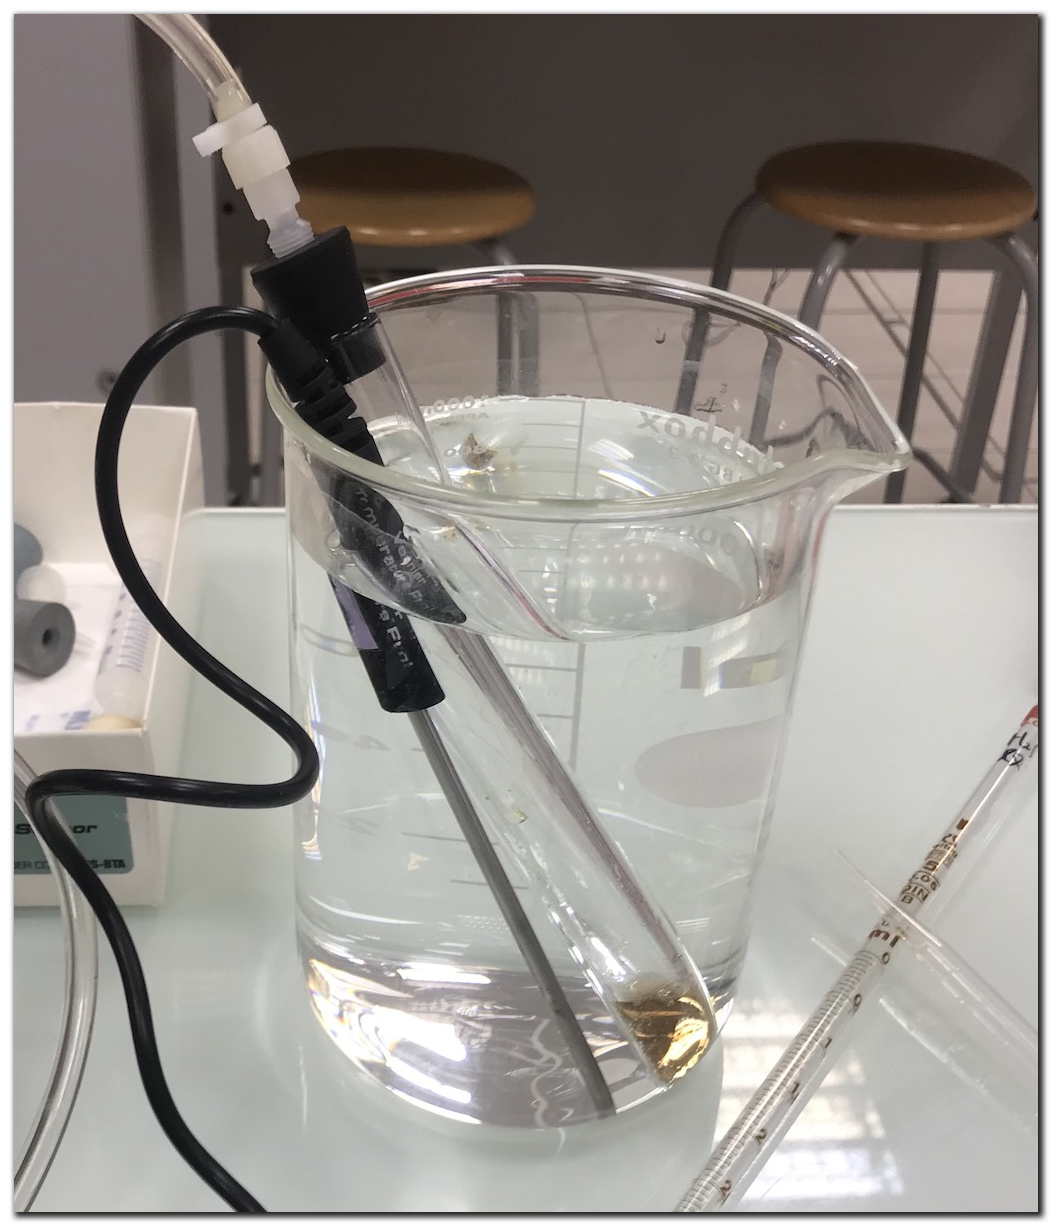
\includegraphics[width=0.36\textwidth]{imgs/setup}
    \caption{Setup of the experiment}
    \label{fig:setup}
\end{figure}


\section*{Raw Data}
\subsection*{Observations}
\begin{itemize}
    \itemsep 0em
    \item \SI{3}{\percent} \ce{H2O2} is a clear, colourless solution. Some fine bubbles can be seen.
    \item Upon the addition of \SI{0.1}{\molar} \ce{FeCl3}, the aqueous catalyst turns from pale yellow to brown, accompanied by a vigorous effervescence after shaking.
    \item 2 trials using \SI{4.00}{\mL} \ce{H2O2} were terminated prematurely, because the rubber stopper popped due to an excessive volume of gas formed.
    \item After about 10 minutes, with the formation of gas becoming less noticeable, the pale yellow colour of \ce{FeCl3} solution returns.
\end{itemize}

\begin{figure}[H]
    \centering
    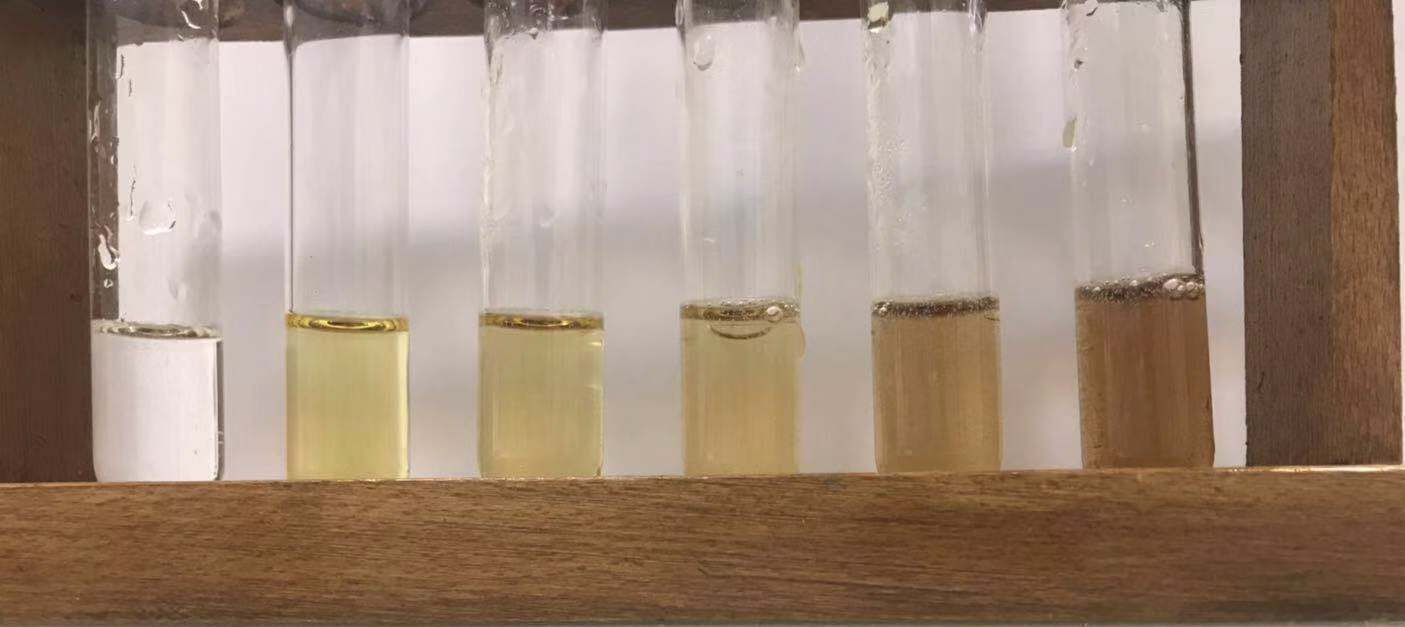
\includegraphics[width=0.8\textwidth]{imgs/colours}
    \caption{(From left to right) hydrogen peroxide, iron(III) chloride, reaction mixtures approximately 12 minutes, 9 minutes, 6 minutes, and 3 minutes after the start of reaction. }
    \label{fig:colours}
\end{figure}

\subsection*{Experimental data}
\begin{figure}[H]
    \centering
    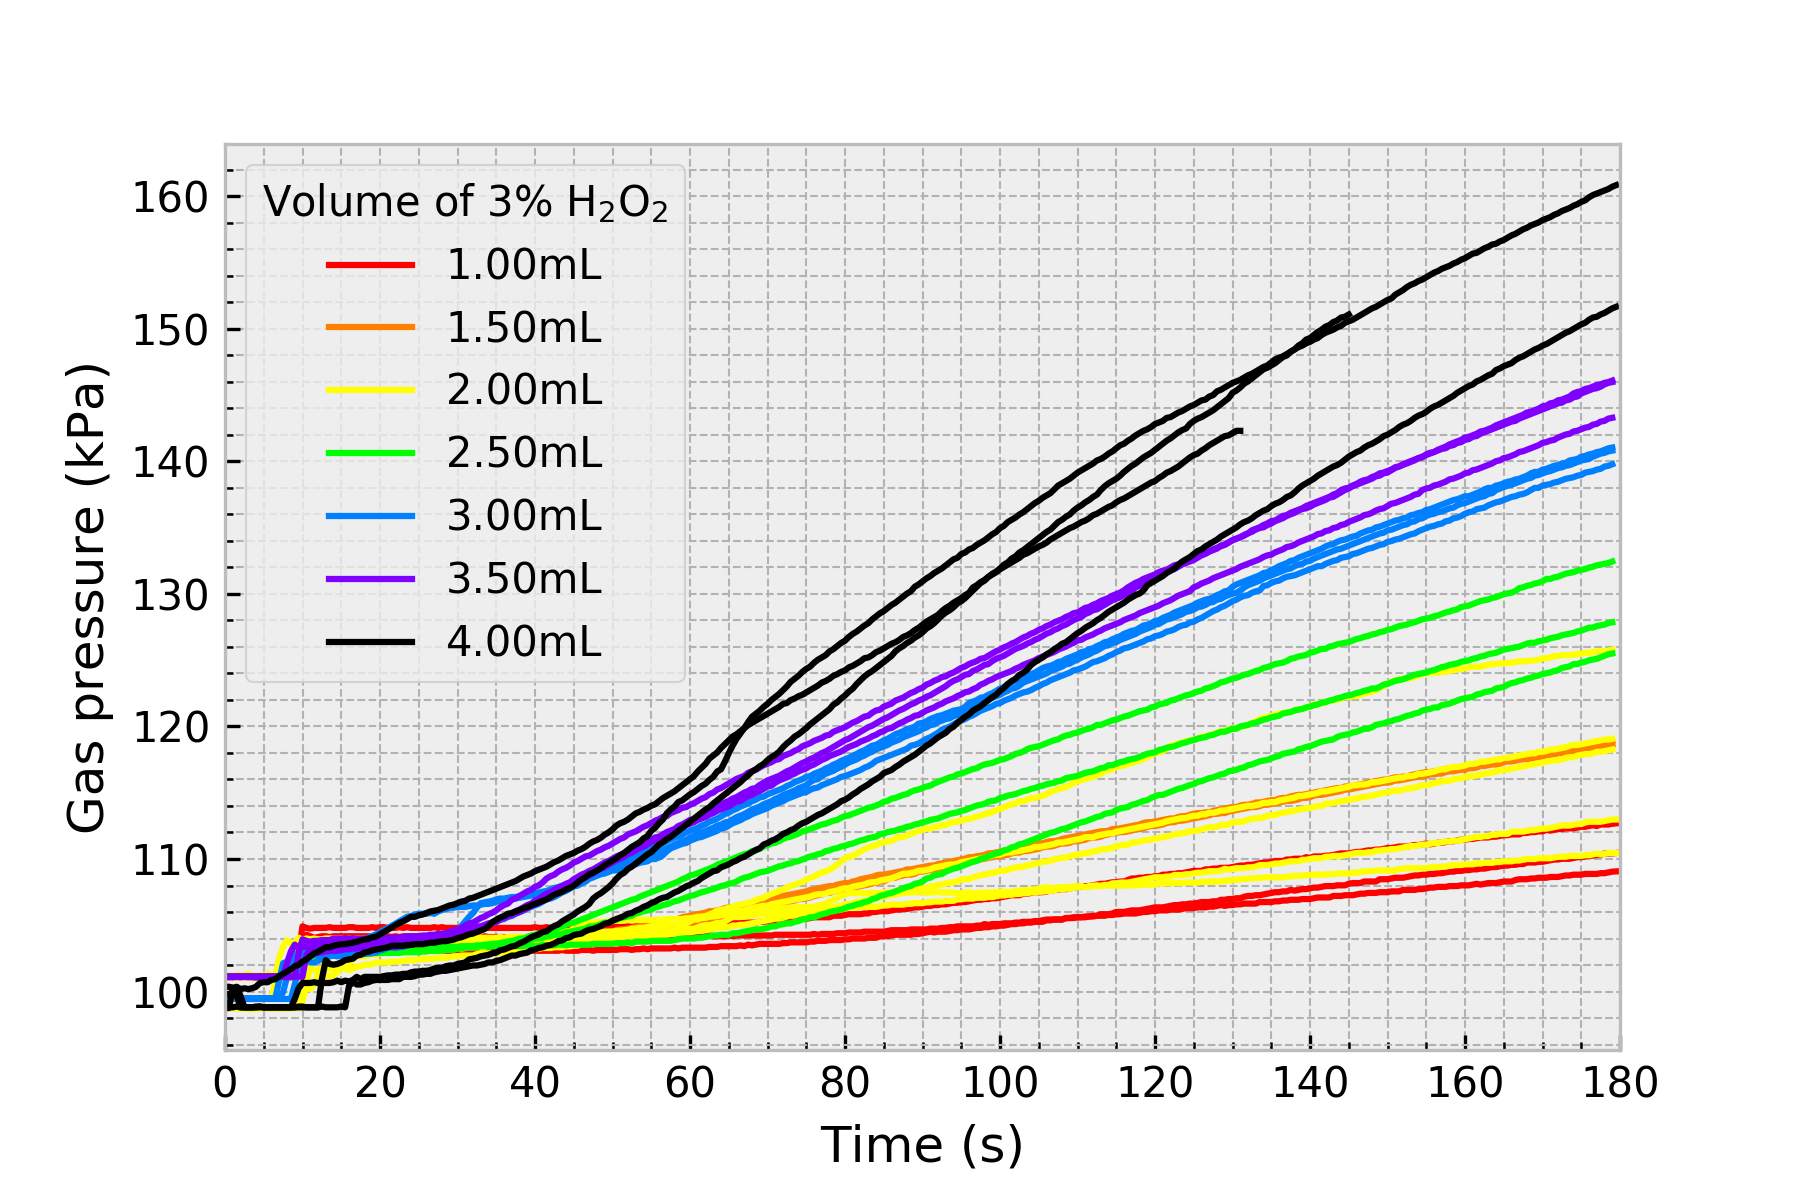
\includegraphics[width=\textwidth]{data/raw_data}
    \caption{Measured gas pressure over time for the decomposition of \ce{H2O2} by \ce{Fe(III)}. $[\ce{Fe^{3+}}] = \SI{0.02}{\molar}$; ambient temperature (\SI{23.2(10)}{\celsius}). }
    \label{fig:raw-data}
\end{figure}

The gas pressure curve generally consists of 3 parts: an initial plateau before sealing the test tube, a slowly increasing curve after inserting the rubber stopper which can be attributed to the dissolution of the oxygen produced, and a linear part where the aqueous oxygen reaches saturation and gaseous oxygen continues to be produced at a mostly consistent rate. Overall, the larger the volume of \SI{3}{\%}  \ce{H2O2} used in the reaction mixture and as such the higher concentration of the \ce{H2O2} reacted, the larger the volume of oxygen gas is formed as measured by the gas pressure at each instant. A deviation from this trend occurs for \SI{2.00}{\mL} of \ce{H2O2}, which may be attributed to the fact that, unlike the other trials, those 4 were all carried out next to the window on a cold winter day resulting in lower reaction rates.

\section*{Processed Data}
Below is a sample calculation for the trials with \SI{3.00}{\mL} of \ce{H2O2} shown by the blue curves in \cref{fig:raw-data}. The initial rate is derived from the first \SI{15}{\s}-long segment of the linear part --- determined by the R$^2$ value of the line of best fit --- using the differential formula \autocite{numerical_method}:
\[ 
    \dv{P}{t} 
    = \dfrac{ P_{ \text{end} } - P_{ \text{start} } }{ t_{ \text{end} } - t_{ \text{start} } }
    \text{ where } t_{ \text{end} } - t_{ \text{start} } = \SI{15.00}{\s}. 
\]

\begin{table}[H]
    \centering
    \caption{Initial rates for reactions with \SI{3.00}{\mL} of \SI{3}{\%} \ce{H2O2}}
    \label{table:calc}
    \begin{tabular}{ | c | c | c | c | }
        \hline
        \multirow{2}{*}{\textbf{Trials}} &
        \multicolumn{2}{ c| }{\textbf{Gas pressure (\si{\kPa}\SI{+-0.01}{\kPa})}}& 
        \multirow{2}{*}{\textbf{Initial rate (\si{\kPa\per\second})}}
        \\ \cline{2-3}
        &
        $t = \SI{91.5}{\second}$ &
        $t = \SI{121.5}{\second}$ &
        \\ \hline
        0 &
        113.96 &
        117.80 &
        0.256
        \\ \hline
        1 &
        119.06 &
        123.19 &
        0.275
        \\ \hline
        2 &
        120.38 &
        124.40 &
        0.268
        \\ \hline
        3 &
        119.92 &
        123.88 &
        0.264
        \\ \hline
        \multicolumn{3}{ | c | }{\textbf{Average}} &
        0.269
        \\ \hline
        \multicolumn{3}{ | c | }{\textbf{Mid-range $= (max + min) / 2$}} &
        0.003
        \\ \hline
    \end{tabular}
\end{table}

Note that the \textbf{accuracy} of \SI{\pm 4}{\kPa} of the gas pressure sensor~\cite{vernier_gas_pressure} is considered to affect the readings consistently, and as such is a systematic error that does not contribute to the uncertainty in the initial rate. Furthermore, the uncertainties arising from the precision of the readings evaluates to 
\begin{align*}
    \Delta \left(\dv{P}{t}\right) 
    &=  \dv{P}{t} 
        \times \left(
            \frac{ 2 \times \SI{0.01}{\kPa} }{P_{ \text{end} } - P_{ \text{start} }}
            + \frac{ 2 \times \SI{0.01}{\s} }{t_{ \text{end} } - t_{ \text{start} }}
        \right)\\
    &= \SI{0.269}{\kPa\per\s} \times \left( \frac{\SI{0.02}{\kPa}}{\SI{0.269}{\kPa\per\s} \times \SI{15.00}{\s}} + \frac{\SI{0.02}{\s}}{\SI{15.00}{\s}} \right)\\
    &= \SI{+-0.002}{\kPa\per\s}
\end{align*}
which is smaller than the mid-range, and is even negligible for some other tirals. Therefore, the uncertainty in the initial rate is determined by the mid-range.

The \SI{3}{\%}(w/w) concentration of \ce{H2O2} means that, proportionally, there is \SI{3}{\g} of \ce{H2O2} per \SI{100}{\g} of solution. In addition, it is indicated on the data sheet \autocite{safety_h2o2} that the density of the solution is \SI{1.01}{\g\per\cm^3}. The molar concentration of the \SI{3}{\%}(w/w) \ce{H2O2} solution is then
\begin{align*}
    % Initial concentration
    [\ce{H2O2}]_{\SI{3}{\%}}
    &= \dfrac{ n(\ce{H2O2}) }{ V(\text{solution}) }\\
    &= \dfrac{ m(\ce{H2O2}) / RFM(\ce{H2O2}) }{ m(\text{solution}) / \rho(\text{solution})}\\
    &= \dfrac{ \SI{3}{\g} / \SI{34.02}{\g\per\mol} } { \SI{100}{\g} / \SI{1.01}{\g\per\cm\cubed} }\\
    &= \SI{8.91E-4}{\mol\per\cm\cubed}\\
    &= \SI{0.891}{\molar}.\\
    % Diluted concentration
    [\ce{H2O2}]
    &= [\ce{H2O2}]_{\SI{3}{\%}} \times \dfrac{ V(\ce{H2O2}) }{ V(\ce{H2O2}) + V(\ce{H2O}) + V(\ce{FeCl3}) }\\
    &= \SI{0.891}{\molar} \times \dfrac{ \SI{3.00}{\mL} }{ \SI{3.00}{\mL} + \SI{1.00}{\mL} + \SI{1.00}{\mL} }\\
    &= \SI{0.534}{\molar}\\
    % Uncertainty in diluted concentration
    \Delta([\ce{H2O2}])
    &= [\ce{H2O2}] \times \fracDeltaP{\ce{H2O2}}\\
    &= [\ce{H2O2}] \times \left(\fracDelta{V(\ce{H2O2})} + \frac{ \Delta V(\ce{H2O2}) + \Delta V(\ce{H2O}) + \Delta V(\ce{FeCl3}) }{ V(\ce{H2O2}) + V(\ce{H2O}) + V(\ce{FeCl3}) }\right)\\
    &= \SI{0.534}{\molar} \times \left(\frac{ 2 \times \SI{0.05}{\mL} }{ \SI{3.00}{\mL} } + \frac{ 2 \times \SI{0.05}{\mL} + \SI{0.05}{\mL} + \SI{0.05}{\mL} }{ \SI{3.00}{\mL} + \SI{1.00}{\mL} + \SI{1.00}{\mL} }\right)\\
    &= \SI{+-0.039}{\molar}
\end{align*}

The figures are calculated in the same figure for the other trials, yielding:

\begin{table}[H]
    \centering
    \caption{Initial rate versus [\ce{H2O2}]. The sample calculation is highlighted in italics. }
    \label{table:data}
    \begin{tabular}{ | c | c | }
        \hline
        \textbf{[\ce{H2O2}]} (\si{\molar}) &
        \textbf{Average initial rate} (\si{\kPa\per\second})
        \\ \hline
        \num{0.178(24)} & \num{0.063(12)}
        \\ \hline
        \num{0.267(28)} & \num{0.106(1)}
        \\ \hline
        \num{0.356(32)} & \num{0.101(49)}
        \\ \hline
        \num{0.445(35)} & \num{0.193(12)}
        \\ \hline
        \textit{\num{0.534(39)}} & \textit{\num{0.269(3)}}
        \\ \hline
        \num{0.623(42)} & \num{0.291(6)}
        \\ \hline
        \num{0.713(46)} & \num{0.366(35)}
        \\ \hline
    \end{tabular}
\end{table}

\section*{Theory}
Two kinetic models are proposed for explaining the experimental data: the rate equation given by a power law, and the Michaelis-Menten equation.

\paragraph{Power law}
This approach assumes that, like for many reactions, the rate equation of the reaction $\ce{ 2 H2O2(aq) ->[Fe^3+] 2 H2O(l) + O2(g) }$ is given by a power law:
\[ \text{rate} = \dv{[\ce{O2(g)}]}{t} = k [\ce{H2O2}]^a [\ce{Fe^3+}]^b. \]
Since [\ce{Fe^3+}] is held constant at \SI{0.02}{\molar}, the above rate equation can be expressed as 
\[ \dv{[\ce{O2(g)}]}{t} = k_{\text{obs}} [\ce{H2O2}]^a \]
where $k_{\text{obs}} = k \times [\ce{Fe^3+}]^b$. Additionally, supposing that the \ce{O2(g)} produced obeys the ideal gas law $P V = n R T$, it can be deduced that $P = \frac{n}{V} \times R T = [\ce{O2(g)}] \times R T$, with $V$ the volume of the test tube being constant. Thus, treating $T$ as a constant,
\begin{align}
    &\dv{P}{t} = \dv{[\ce{O2(g)}]}{t} \times R T \nonumber\\
    \iff &\dv{P}{t} = k_\text{obs} [\ce{H2O2}]^a \times R T \nonumber\\
    \iff &\dv{P}{t} = k_\text{obs}' [\ce{H2O2}]^a \text{ where } k_\text{obs}' = k_\text{obs} \times R T.\label{eq:rateEq}
\end{align}
The parameters $a$ and $k_{\text{obs}}'$ are then determined using MATLAB's curve fitting toolbox~\cite{matlab}.

\paragraph{Michaelis-Menten equation}
This approach is typically applied to model single-substrate enzyme-catalysed reactions, namely, the sequence of elementary reactions
\[
\ce{E + S <=>[ k_f ][ k_r ] ES ->[ k_{\text{cat}} ] E + P}
\]
where \ce{E}, \ce{S}, and \ce{P} are respectively the enzyme, the substrate, and the product. In this study, it is hypothesised that \ce{Fe^3+}, \ce{H2O2}, and \ce{O2} respectively play these roles.

Since the enzyme acts as a catalyst and is not consumed during the course of the reaction, it is admitted that $\ce{[E]_0} = \ce{[E] + [ES]}$ where $\ce{[E]_0}$ is the initial enzyme concentration, or equivalently, 
\[
\ce{[E]} = \ce{[E]_0 - [ES]}.
\]

A quasi-steady-state of the concentration of the intermediate \ce{ES} is assumed; i.e., 
\begin{align*}
    &\ce{k_f [E][S] - k_r [ES] - k_{\text{cat}} [ES] = 0}\\
    \iff &\ce{k_f ([E]_0 - [ES]) [S] - (k_r + k_{\text{cat}}) [ES] = 0}\\
    \iff &\ce{k_f [E]_0 [S] = (k_f [S] + k_r + k_{\text{cat}})[ES]}\\
    \iff &\ce{[ES] = \frac{k_f [E]_0 [S]}{k_f [S] + (k_r + k_{\text{cat}})}}
    = \ce{\frac{[E]_0 [S]}{[S] + K_m}}
\end{align*}
where $K_m = \dfrac{k_r + k_\text{cat}}{k_f}$ is known as the Michaelis constant. Finally, from $\ce{ES ->[k_{\text{cat}}] E + P}$, the rate of product of product formation is given by
\begin{align}
    \dv{\ce{[P]}}{t} &= k_{\text{cat}} \times \ce{[ES]} = k_{\text{cat}} \times \frac{\ce{[E]_0[S]}}{\ce{[S]} + K_m}
\nonumber\\
    \iff \dv{P}{t} &= k_{\text{obs}} \times \frac{\ce{[S]}}{\ce{[S]} + K_m}\label{eq:mm}
\end{align}
where $k_{\text{obs}} = k_\text{cat} \ce{[E]_0} \times R T$. The parameters $k_{\text{obs}}, K_m$ along with an y-intercept to account for systematic errors are then determined using MATLAB's curve fitting toolbox~\cite{matlab}.

\section*{Results}

\begin{figure}[H]
    \centering
    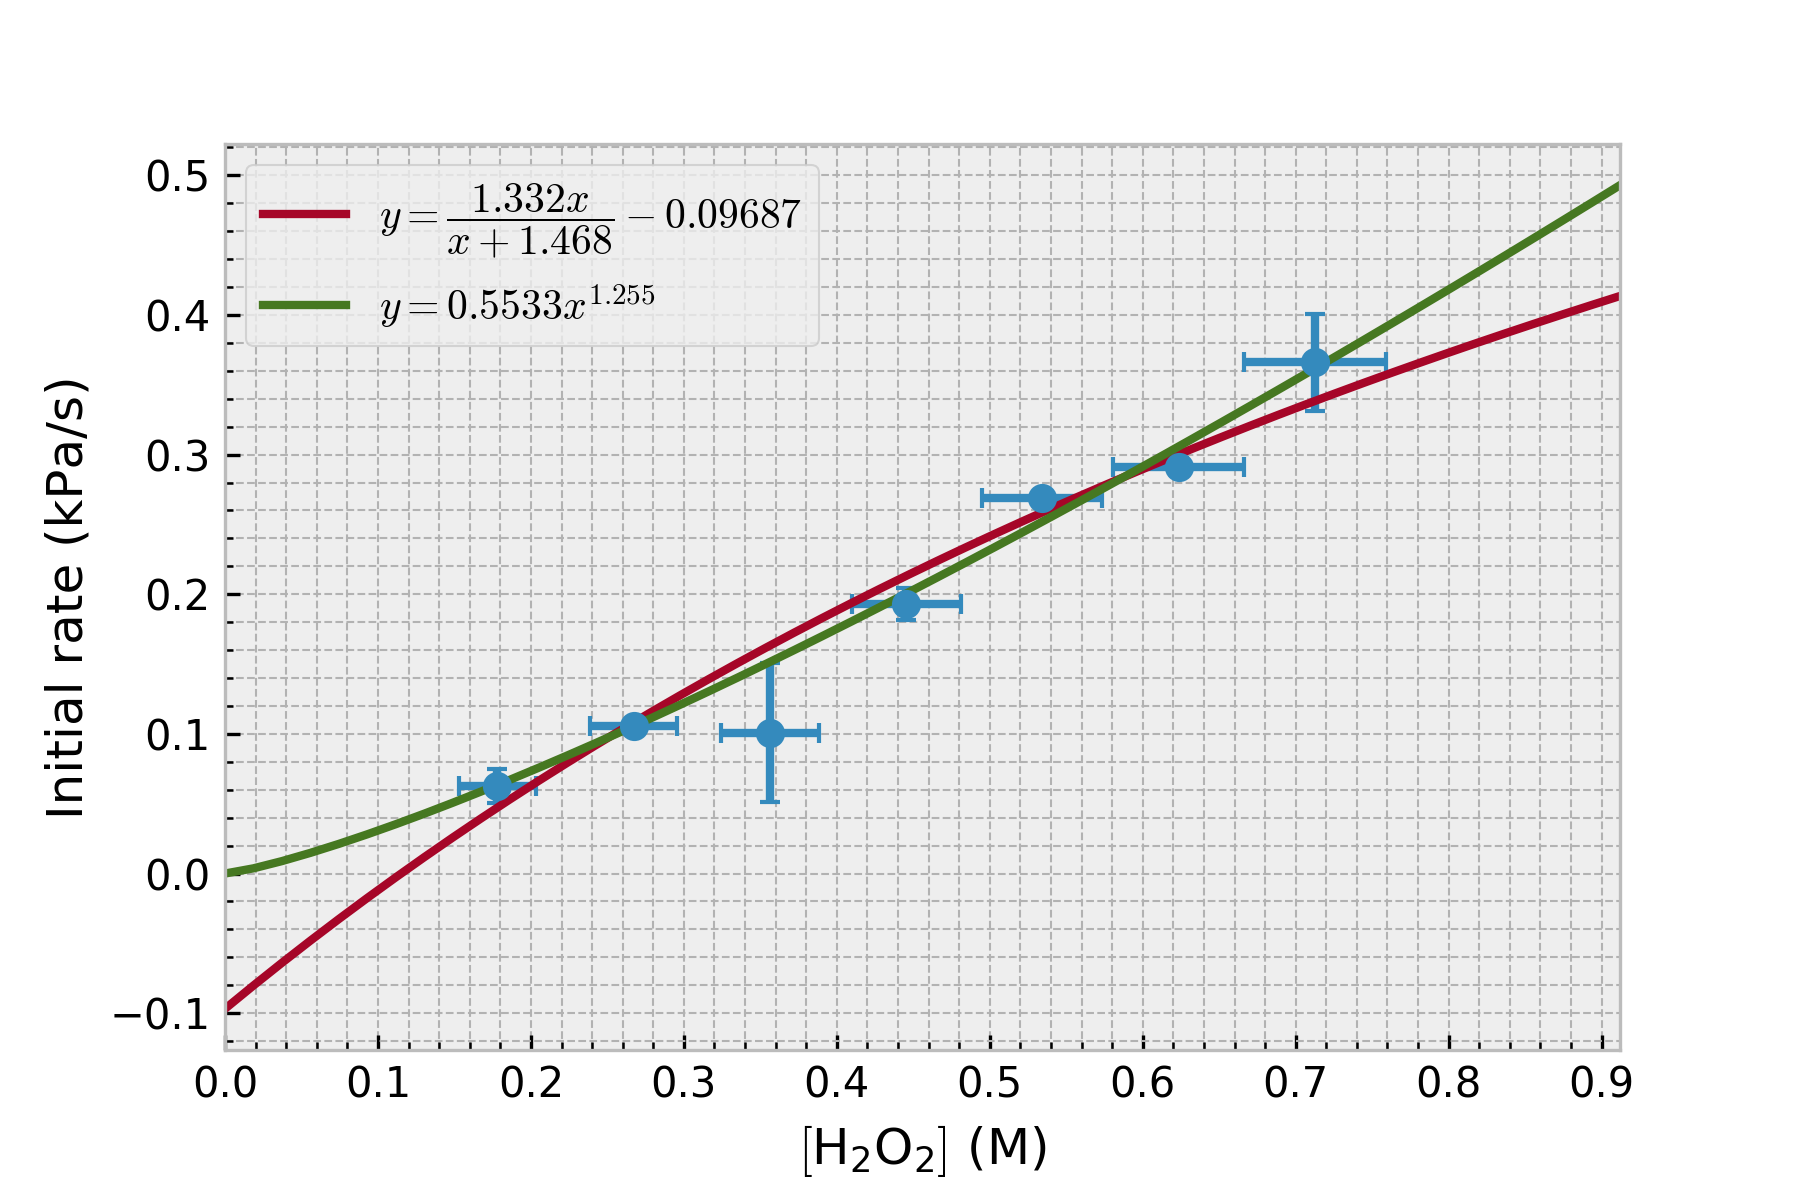
\includegraphics[width=\textwidth]{data/processed_data}
    \caption{Initial rate versus [\ce{H2O2}]. [\ce{Fe^3+}] = \SI{0.02}{\molar}; ambient temperature (\SI{23.3(10)}{\celsius}). \Cref{eq:rateEq}, the rate equation is shown in green; \cref{eq:mm}, the Michaelis-Menten equation, is shown in red. }
    \label{fig:processed-data}
\end{figure}

At the exception of the \SI{2.00}{\mL} (or \SI{0.356}{\molar}) \ce{H2O2} trials, both curves pass through all the data points within the relatively tolerant margins of error. Hence, the experimental data appear to support both the power law formulation and the Michaelis-Menten model. However, the respective characteristics of the two kinetic models should be discussed with reference to the data.

\Cref{fig:processed-data} shows that, with the power law formulation of the rate equation, the ferric ion catalysed decomposition reaction of hydrogen peroxide is of order $1.255$ with respect to~\ce{H2O2}. Firstly, the reaction can be considered as pseudo-first order, as reported by de Laat and Gallard~\cite{de_laat} for lower $\ce{Fe(III)}$ catalyst concentrations and by Abbot and Brown~\cite{pseudo_first_order} under alkaline conditions. Moreover, since $1.255 \approx \frac{5}{4}$, it can be considered as a fractional order that often arises in chain reactions where intermediates are involved~\cite{atkins}. Nevertheless, such orders only indicate that intermediate steps exist, but does not offer insight into the concrete reaction mechanism.

On the other hand, the Michaelis-Menten equation is derived from the rates of the proposed reaction steps. The model postulates that the decomposition of \ce{H2O2} consists of a reversible binding of \ce{Fe(III)} with \ce{H2O2} forming \ce{Fe(III)-H2O2} intermediates, and an irreversible production of \ce{O2} from \ce{Fe(III)-H2O2}. Tachiev et al.~\cite{tachiev} proposed a similar mechanism for the decomposition of \ce{H2O2} catalysed by \ce{Fe(II)}; Francis et al.~\cite{Fe_mm} empirically determined a rate equation that takes the same form as \cref{eq:mm} for \ce{Fe(III)} complexes. It is further assumed that the products do not affect the reaction rates; i.e., \ce{H2O} and \ce{O2} do not act as a catalyst or an inhibitor in any of the steps. Given that \ce{O2} is formed at a very controlled rate, even if the concentration of \ce{O2} has an impact on the rates, \ce{[O2]} will be negligible at the start of the reaction. As such, only the initial rates are considered. On the other hand, the instantaneous establishment of the quasi-steady-state requires that~\cite{mathematical_biology} \[ \frac{\ce{[E]_0}}{\ce{[S]} + K_m} \ll 1 . \] In this study, $\ce{[E]_0} = \SI{0.02}{\molar}$ across all trials; $\ce{[S]}$ varies from \SI{0.178}{\molar} to \SI{0.713}{\molar}; $K_m = \SI{1.468}{\molar}$ as seen in \cref{fig:processed-data}. Clearly, $\ce{[E]_0} \ll \ce{[S]} + K_m$ and the condition is met.

Attention should be paid to the negative y-intercept of $-0.09687$ of the Michaelis-Menten curve in \cref{fig:processed-data}. A negative reaction rate does not carry any chemical meaning; the y-intercept should therefore be due to systematic errors which will be discussed below.

A survey of the literature revealed many different reaction mechanisms (\cite{pseudo_first_order} \cite{Fe_mm} \cite{de_laat} \cite{tachiev}) subject to a range of factors -- the initial concentration of \ce{H2O2}, the initial concentration of \ce{Fe(III)} catalyst, pH of the solution, etc. Unfortunately, no publication that coincides with the circumstances studied in this experiment was found to validate the results. That said, despite the limited precision due to the apparatus used in a school laboratory, this study can serve to test the applicability of the proposed models under a wider range of conditions.

To conclude, with the available experimental data, both the power law formulation and the Michaelis-Menten model are plausible mechanisms for the decomposition of hydrogen peroxide in presence of \ce{Fe^3+} ion catalysts. Nonetheless, at higher \ce{H2O2} concentrations, the Michaelis-Menten model predicts that the initial rate will be nearly zero-order with respect to hydrogen peroxide, while the power law predicts that the initial rate will grow exponentially. As such, further trials with higher \ce{H2O2} concentrations (e.g., $\ce{[H2O2]}~\geq~\SI{1.0}{\molar}$) need to be conducted to verify the validity of either model. Given the complex nature of the catalysis process, however, it is very likely that neither model will be able to fully explain the dependence of the initial rate on \ce{H2O2} concentration.

\section*{Evaluation}
At last, the systematic errors and the underlying assumptions should be addressed.

Concerning the execution of the experiment, after each trial, each test tubes is rinsed and cleaned, but some drops of water can be seen on the wall of the tube near the bottom. In effect, the water drops increase the total volume of the reaction mixture and decrease the effective concentration of \ce{H2O2} that is reacted. Graphically, the effect of this systematic error is reflected in \cref{fig:processed-data} by data points that are shifted horizontally to the right compared to their actual positions. As such, considering the corrected values of \ce{[H2O2]} will to an extent account for the negative y-intercept, and make the Michaelis-Menten model a more reasonable explanation of the reaction mechanism. In hindsight, avoiding such an error is in fact fairly simple -- it suffices to either use other clean, dry test tubes, or to rinse the test tubes with acetone which forms a mixture with water that would quickly evaporate.

The data processing also relies on several assumptions. To begin with, it is accepted that the concentration of oxygen gas can be calculated from the gas pressure using the ideal gas equation, $P V = n R T$, where $V$ and $T$ are considered as constants. One concern is that, although all the $6$ test tubes used are labelled to be \SI{18x150}{\mm}, not calibrating and not holding down the rubber stopper tightly enough may result in different volumes in practice. Nonetheless, since it is the rate of change in oxygen concentration that is considered, we have $\dv{P}{t} = \dv{\ce{[O2(g)]}}{t} \times RT$ as shown before, which does not depend on $V$, regardless of whether it is a constant. The variation of $T$, however, is then an actual concern. Even though dividing the gas pressure by temperature and then calculating the rate of change appears to make the results more accurate, such an operation turns out to be unnecessary and problematic to a certain degree. As indicated in the caption of \cref{fig:raw-data}, the temperature at which the trials are carried out is \SI{23.2(10)}{\celsius}, or \SI{296.4(10)}{\kelvin}. The change in gas pressure only varies between \SI{0.063}{\kPa\per\second} and \SI{0.366}{\kPa\per\second} (see \cref{table:data}). A variation in $T$ of \SI{+-1.0}{\kelvin} will therefore not lead to a significant discrepancy; in addition, dividing small $\dv{P}{t}$ values by relatively large $RT$ values results in small figures that are very close to $0$, making calculations prone to numeric errors and exposing the sensitive fitting process to measurement errors. Also, it is assumed that the initially slow increase in gas pressure is due to oxygen being dissolved in the solution. To confirm that this occurs, it is possible to measure the oxygen saturation of the solution with a dissolved oxygen probe before and after the reaction. Furthermore, the validity of the ideal gas law when applied to oxygen is another problem. A modified equation taking into account the volume of the oxygen gas molecules and the intermolecular interactions is \cite{weast_1972} \[ P = \frac{nRT}{V - 0.03186n} - \frac{1.382n^2}{V^2} .\]
It should be noted that since $n \ll V$ and is very close to zero, the above equation roughly reduces to the ideal equation $P = \frac{nRT}{V}$, meaning that the calculations are valid.

There are several remarks to be made about the homogeneous catalysis mechanism. It is admitted that \ce{Fe(III)} is not consumed during the reaction; indeed, the qualitative observations confirm that the solution takes the pale yellow colour of \ce{FeCl3} both at the start and at the end of the reaction. It is further assumed that \ce{FeCl3} dissociates into \ce{Fe^3+} and \ce{Cl-} ions in water, and the latter play no role in the decomposition of \ce{H2O2}. De Laat and Gallard \cite{de_laat} reported a significant variation of the initial rate depending on the pH of the solution. Although there was no sight of \ce{Fe(OH)3} precipitate which indicates an acidic pH where the \ce{H2O2} is catalytically decomposed by \ce{Fe(III)} \cite{de_laat}, it is good practice to control the pH of the solution by taking measures with a pH probe before and after the reaction. Nevertheless, using the method proposed in this study, it cannot be determined whether the intermediate steps involve the formation of radicals such as \ce{OH.} and \ce{OOH.} \cite{detection} \cite{de_laat} \cite{tachiev}, which can be detected voltammetrically \cite{detection} or spectrometrically \cite{de_laat}. 

Indeed, it is possible to measure the initial rates using other methods. The gas pressure approach presented in this study is advantageous in that it is easy to set up in a school laboratory, and allows rapid data collection. Its shortcomings include possible gas leaks as a systematic error that causes slower rates to be measured and the inability to determine the reaction intermediates. Instead, a batch reactor can be used; samples are taken after a fixed amount of time, and hydrogen peroxide concentration can be determined iodometrically or spectrometrically with \ce{TiCl4} \cite{de_laat}. The results obtained using different approaches can then be compared to enable a more accurate conclusion to be made.

Apart from checking whether the proposed models are still valid for a broader range of \ce{[H2O2]} values, another way to further this study is to determine the activation energy of \ce{Fe(III)}-catalysed decomposition of \ce{H2O2}. This can be achieved by fixing the reactant concentrations and varying the temperature; the activation energy can then be calculated from the y-intercept using the Arrhenius plot. Similarly, it is possible to determine the activation energy of other transition metal catalysts, complexed or free (as long as the catalysis is homogeneous). A comparison of the kinetic values could then possibly shed insight on the complex homogeneous catalysis mechanism concerning hydrogen peroxide.

% Bibliography
\clearpage
\thispagestyle{empty}
\printbibliography
\thispagestyle{empty}

\end{document}
